\section{Clase 21}
\subsection{Dinámica de líquidos y gas}
Procesos de expansión
\begin{enumerate}
	\item \textbf{Isotrópico}: La entropía se conserva ($\Delta S=0$).
	\item \textbf{Aislado}: No hay transferencia de calor con el exterior.
	\item \textbf{Adiabático}: Expansión lenta.


\underline{Nota:} Que un proceso sea aislado y adiabárico implica que es isoentrópico. Generalmente adiabático se usa para significar $\Delta S=0$, en este caso se asume un sistema aislado.

\item \textbf{Abrupta o instantánea}: $\Delta E=0$ (No hay tiempo de intercambiar energía con el exterior) y $\Delta S\neq 0$.
\end{enumerate}

\underline{Importante:} Una expansión aislada o proceso aislado (sin transferencia de calor) puede ser adiabático, abrupta o algo intermedio. En el primer caso $\Delta S=0$ y en le segundo $\Delta E=0$.

\begin{ej}
	Consideremos una camara con un pistón 
	\begin{figure}[h!]
		\centering
		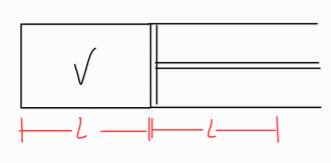
\includegraphics[scale=0.5]{fig/21-img.png}
	\end{figure}
\end{ej}
  
Supongamos que la cámara contiene $N$ moléculas de un gas ideal monoatómico a temperatura $T$ ocupando un volúmen $V$ Asuma que la cámara está aislada del entorno.
\begin{enumerate}
	\item Si se retrotrae el émbolo hasta aumentar el volúmen al doble de fora lenta (adiabático), encuentre el cambio de energía y entropía del sistema.
	\item Si ahora el proceso es instantáneo, encuentre el cambio de energía y entropía del sistema
\end{enumerate}

\begin{sol}
\begin{enumerate}
\item 	

	Por enunciado 
	\begin{equation}
  \dd S=0\Rightarrow\boxed{ \Delta S=0}
\end{equation}
Usamos la primera ley
\begin{align}
  \dd E&=T\dd S-P\dd V+\m\dd N,\qquad \dd S=0,\qquad \dd N=0\\
  \dd E&=-P\dd V
\end{align}
Podríamos usar que
\begin{align}
  PV&=N\k T\\
  P&=\frac{N\k T}{V}
\end{align}
Pero 
\begin{align}
  \dd T&\neq 0\implies \dd E\neq 0\\
  E&=\frac{3}{2}N\k T
\end{align}
es decir, $E$ depende de $T$.

Consideremos la entropía de un gas ideal monoatómico
\begin{align}
  F&=E-TS=-\k T\ln (\zc )\\
  S&=\frac{E}{T}+\k \ln(\zc )
\end{align}
además
\begin{equation}
  \zc =\frac{1}{N!}V^N\left(\frac{m\k T}{2\p\hbar^2}\right)^{3N/2}
\end{equation}
y
\begin{equation}
  E=\frac{3}{2}N\k T
\end{equation}
Reemplazando y usando Stirling
\begin{equation}
  S=\frac{3}{2}N\k +\k \left(-N\ln(N)+N+N\ln (V)+\frac{3}{2}N\ln\left(\frac{m\k T}{2\p\hbar^2}\right)^{3/2}\right)
\end{equation}
Entonces la entropía del gas ideal monoatómico
\begin{equation}
\boxed{  S=N\k \left(\frac{5}{2}+\ln\left(\frac{V}{N}\left(\frac{m\k T}{2\p\hbar^2}\right)\right)^{3/2}\right)}
\end{equation}
Ahora,
\begin{equation}
  \eval{\Delta S}_N=0
\end{equation}
implica
\begin{equation}
  V_1T_1^\gamma =V_2T_2^\gamma
\end{equation}
y el $\gamma$ que cumple que $\Delta s=0$
\begin{align}
  V_1T_1^{3/2}&=V_2T_2^{3/2}\\
  \frac{V_2}{V_1}&=\left(\frac{T_1}{T_2}\right)^{3/2}=2\\
  T_2&=2^{-2/3}T_1\\
  \frac{T_2}{T_1}&=2^{-2/3}
\end{align}
y usando la energía del gas ideal monoatómico podemos encontrar $\Delta E$,
\begin{equation}
  \frac{E_2}{E_1}=2^{-2/3}
\end{equation}
\begin{equation}
  \Delta E=E_2-E_2
\end{equation}
\begin{equation}
\boxed{  \Delta E=(2^{-2/3}-1)E_1}
\end{equation}
\item 
En este caso
\begin{equation}
  \Delta E=0
\end{equation}
y $\Delta S\neq 0$. Ahora como $\dd E=0 \implies \dd T=0$.

Podemos usar que
\begin{align}
  T\dd S&=P\dd V\\
  \dd S&=\frac{P}{T}\dd V\qquad P(V)=\frac{N\k T}{V}
\end{align}
integramos y obtenemos
\begin{align}
  \Delta S&=\int_{V_1}^{V_2}\frac{N\k }{V}\dd V\\
  &=N\k \ln\left(\frac{V_2}{V_1}\right)
\end{align}
\begin{equation}
\boxed{  \Delta S=N\k \ln(2)}
\end{equation}









\end{enumerate}




































\end{sol}